\mxfront{stmg-bank-d}

% -----------------------------------------------------------------------------
% Chapitre 7 -- Variables aléatoires discrètes et loi binomiale
% -----------------------------------------------------------------------------
\mxexdef{47}{Loi d'un gain et espérance}{%
Pour le lancement d'un nouveau parfum, une enseigne de cosmétiques vend à ses clients, au prix de $3$~€, un ticket à gratter. Les tickets sont imprimés en carnets de $25$ : dans chaque carnet, $16$ tickets sont perdants, $6$ tickets donnent droit à un bon d'achat de $6$~€ et $3$ tickets donnent droit à un bon d'achat de $13$~€. Un client achète un ticket choisi au hasard dans un carnet neuf.

On note $G$ la variable aléatoire égale au gain net du client, en euros, c'est-à-dire la valeur du bon obtenu diminuée du prix du ticket (un gain négatif est une perte).
\begin{enumerate}
\item Quelles sont les valeurs prises par $G$ ?
\item Recopier et compléter le tableau suivant, qui donne la loi de probabilité de $G$.
\begin{center}
\mxarraystretch{1.4}
\begin{tabular}{|l|*{3}{p{1.7cm}|}}
\hline
Valeur $g_i$ de $G$ & & & \\
\hline
$P(G=g_i)$ & & & \\
\hline
\end{tabular}
\end{center}
\item Calculer l'espérance $E(G)$. Que peut-on en dire du point de vue du client ? et de l'enseigne ?
\item L'enseigne souhaite gagner en moyenne $\num{0,40}$~€ par ticket vendu, sans modifier la composition des carnets. À quel prix doit-elle vendre le ticket ?
\end{enumerate}
}{%
\begin{enumerate}
\item Un ticket perdant donne $G=0-3=-3$ ; un bon de $6$~€ donne $G=6-3=3$ ; un bon de $13$~€ donne $G=13-3=10$. Donc $G$ prend les valeurs $-3$, $3$ et $10$.
\item Le ticket est choisi au hasard parmi $25$ tickets : situation d'équiprobabilité.
\[
\begin{array}{|l|c|c|c|}\hline
g_i&-3&3&10\\\hline
P(G=g_i)&\dfrac{16}{25}=\num{0,64}&\dfrac{6}{25}=\num{0,24}&\dfrac{3}{25}=\num{0,12}\\\hline
\end{array}
\]
Contrôle : $\num{0,64}+\num{0,24}+\num{0,12}=1$.
\item $E(G)=-3\times\num{0,64}+3\times\num{0,24}+10\times\num{0,12}=-\num{1,92}+\num{0,72}+\num{1,20}=0$.
L'espérance est nulle : sur un grand nombre de tickets, le client ne gagne ni ne perd en moyenne ; le jeu est équitable. L'enseigne ne gagne rien en moyenne sur les tickets eux-mêmes : l'opération ne sert qu'à attirer la clientèle.
\item Notons $B$ la valeur du bon. $E(B)=0\times\num{0,64}+6\times\num{0,24}+13\times\num{0,12}=\num{1,44}+\num{1,56}=3$~€. Si le ticket coûte $c$ euros, le gain net du client est $B-c$ et son espérance vaut $3-c$ (chaque valeur de $G$ est diminuée de $c$). On veut $3-c=-\num{0,40}$, donc $c=\num{3,40}$~€.
Vérification : les valeurs deviennent $-\num{3,40}$, $\num{2,60}$, $\num{9,60}$ et $-\num{3,40}\times\num{0,64}+\num{2,60}\times\num{0,24}+\num{9,60}\times\num{0,12}=-\num{2,176}+\num{0,624}+\num{1,152}=-\num{0,40}$.
\end{enumerate}
}{5}

\mxexdef{48}{Reconnaître une loi binomiale, n = 2}{%
Sur une grande plateforme de vente en ligne, $\pc{12}$ des colis expédiés font l'objet d'un retour par le client. Le service qualité choisit au hasard deux colis expédiés. Le nombre de colis expédiés est suffisamment grand pour que l'on puisse assimiler ce choix à deux tirages au hasard avec remise.

On note $R$ l'événement « le colis fait l'objet d'un retour » et $X$ la variable aléatoire égale au nombre de colis retournés parmi les deux colis choisis.
\begin{center}
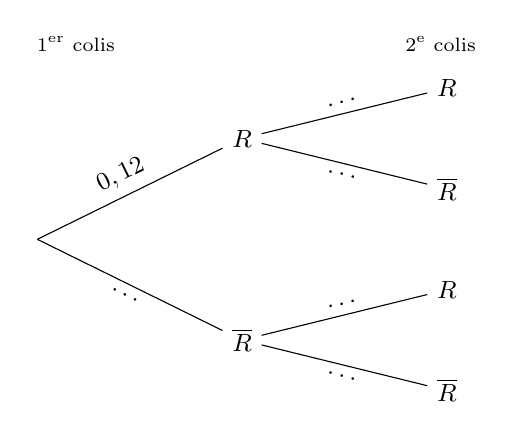
\begin{tikzpicture}[font=\small,x=26mm,y=8mm]
\coordinate (O) at (0,0);
\node (R1) at (1,1.6) {$R$};
\node (N1) at (1,-1.6) {$\overline R$};
\node (RR) at (2,2.4) {$R$};
\node (RN) at (2,0.8) {$\overline R$};
\node (NR) at (2,-0.8) {$R$};
\node (NN) at (2,-2.4) {$\overline R$};
\draw (O)--node[above,sloped]{$\num{0,12}$}(R1);
\draw (O)--node[below,sloped]{$\dots$}(N1);
\draw (R1)--node[above,sloped]{$\dots$}(RR);
\draw (R1)--node[below,sloped]{$\dots$}(RN);
\draw (N1)--node[above,sloped]{$\dots$}(NR);
\draw (N1)--node[below,sloped]{$\dots$}(NN);
\node[anchor=west,font=\scriptsize] at (-0.05,3.1) {1\textsuperscript{er} colis};
\node[anchor=west,font=\scriptsize] at (1.75,3.1) {2\textsuperscript{e} colis};
\end{tikzpicture}
\end{center}
\begin{enumerate}
\item Recopier et compléter l'arbre pondéré ci-dessus.
\item Justifier que $X$ suit une loi binomiale et préciser ses paramètres.
\item Calculer $P(X=0)$, $P(X=1)$ et $P(X=2)$. Pour $P(X=1)$, préciser combien de chemins de l'arbre réalisent l'événement $\{X=1\}$.
\item En déduire, de deux façons différentes, la probabilité qu'au moins un des deux colis fasse l'objet d'un retour.
\end{enumerate}
}{%
\begin{enumerate}
\item Premier niveau : $P(R)=\num{0,12}$ et $P(\overline R)=1-\num{0,12}=\num{0,88}$. Les tirages étant assimilés à des tirages avec remise, le second niveau reprend les mêmes probabilités : $\num{0,12}$ vers $R$ et $\num{0,88}$ vers $\overline R$ sur chacune des deux branches.
\item On répète $2$ fois, de façon identique et indépendante (tirage assimilé à un tirage avec remise), une épreuve de Bernoulli dont le succès « le colis est retourné » a pour probabilité $\num{0,12}$. La variable $X$ compte le nombre de succès : $X$ suit la loi binomiale $\mathcal B\pt{2;\num{0,12}}$.
\item $P(X=0)=\num{0,88}^2=\num{0,7744}$.
Deux chemins réalisent $\{X=1\}$ : $(R,\overline R)$ et $(\overline R,R)$, d'où $P(X=1)=2\times\num{0,12}\times\num{0,88}=\num{0,2112}$.
$P(X=2)=\num{0,12}^2=\num{0,0144}$.
Contrôle : $\num{0,7744}+\num{0,2112}+\num{0,0144}=1$.
\item « Au moins un retour » est l'événement $\{X\geqslant1\}$.
Par addition : $P(X\geqslant1)=P(X=1)+P(X=2)=\num{0,2112}+\num{0,0144}=\num{0,2256}$.
Par l'événement contraire : $P(X\geqslant1)=1-P(X=0)=1-\num{0,7744}=\num{0,2256}$.
Il y a donc environ $\pc{22,6}$ de chances qu'au moins un des deux colis soit retourné.
\end{enumerate}
}{5}

\mxexdef{49}{Triangle de Pascal et loi B(n ; 1/2)}{%
Une boutique en ligne teste deux présentations de sa page d'accueil (test A/B) : à chaque nouveau visiteur, le site affiche au hasard la version A ou la version B, avec la même probabilité $\dfrac12$, indépendamment des autres visiteurs. On observe les $7$ prochains visiteurs et on note $X$ la variable aléatoire égale au nombre de visiteurs à qui la version B est affichée.
\begin{enumerate}
\item Justifier que $X$ suit une loi binomiale et préciser ses paramètres.
\item Construire le triangle de Pascal jusqu'à la ligne $n=7$.
\item Lire $\binom73$ dans le triangle et interpréter ce nombre dans le contexte. Calculer $P(X=3)$ sous forme de fraction, puis arrondie à $10^{-3}$. Interpréter le résultat.
\item Calculer la probabilité qu'au moins $5$ des $7$ visiteurs voient la version B (fraction, puis arrondi à $10^{-3}$).
\end{enumerate}
}{%
\begin{enumerate}
\item Chaque visiteur constitue une épreuve de Bernoulli de succès « la version B est affichée », de probabilité $\dfrac12$. Les $7$ épreuves sont identiques et indépendantes, et $X$ compte les succès : $X\sim\mathcal B\left(7;\dfrac12\right)$.
\item
\begin{center}
\begin{tabular}{c|*{8}{c}}
$n$&\multicolumn{8}{l}{coefficients $\binom nk$ pour $k=0,\dots,n$}\\\hline
$0$&1\\
$1$&1&1\\
$2$&1&2&1\\
$3$&1&3&3&1\\
$4$&1&4&6&4&1\\
$5$&1&5&10&10&5&1\\
$6$&1&6&15&20&15&6&1\\
$7$&1&7&21&35&35&21&7&1
\end{tabular}
\end{center}
Chaque coefficient intérieur est la somme du coefficient situé juste au-dessus et du coefficient placé à gauche de ce dernier (par exemple $\binom73=\binom62+\binom63=15+20=35$).
\item $\binom73=35$ : il y a $35$ suites différentes de $7$ affichages contenant exactement $3$ fois la version B. Chaque suite a pour probabilité $\left(\dfrac12\right)^3\left(\dfrac12\right)^4=\dfrac1{128}$, donc
$P(X=3)=\dfrac{35}{128}\approx\num{0,273}$. Dans environ $\pc{27}$ des séries de $7$ visiteurs, exactement $3$ voient la version B.
\item $P(X\geqslant5)=P(X=5)+P(X=6)+P(X=7)=\dfrac{21+7+1}{128}=\dfrac{29}{128}\approx\num{0,227}$.
\end{enumerate}
}{5}

\mxexdef{50}{Probabilités binomiales, triangle jusqu'à n = 8}{%
Dans un cabinet médical, on estime qu'un patient ayant pris rendez-vous en ligne se présente effectivement à sa consultation avec une probabilité de $\num{0,9}$. Un matin, un médecin a $8$ rendez-vous pris en ligne. On note $X$ la variable aléatoire égale au nombre de patients qui se présentent parmi ces $8$. On admet que $X$ suit une loi binomiale.

Les probabilités seront arrondies à $10^{-3}$.
\begin{enumerate}
\item Donner les paramètres $n$ et $p$ de la loi de $X$.
\item Calculer la probabilité des événements suivants :
$A$ : « les $8$ patients se présentent » ; $B$ : « au moins un patient ne se présente pas ».
\item Construire le triangle de Pascal jusqu'à la ligne $n=8$. En déduire $\binom86$, puis la probabilité de l'événement $C$ : « exactement $6$ patients se présentent ».
\item Traduire par une phrase l'événement $\{X=7\}$, puis calculer $P(X=7)$.
\end{enumerate}
}{%
\begin{enumerate}
\item $n=8$ et $p=\num{0,9}$ : $X\sim\mathcal B\pt{8;\num{0,9}}$.
\item $P(A)=P(X=8)=\num{0,9}^8\approx\num{0,430}$.
$B$ est l'événement contraire de $A$ : $P(B)=1-\num{0,9}^8\approx\num{0,570}$.
\item Ligne $8$ du triangle (obtenue à partir de la ligne $7$ : $1,\allowbreak 7,\allowbreak 21,\allowbreak 35,\allowbreak 35,\allowbreak 21,\allowbreak 7,\allowbreak 1$) : $1,\allowbreak 8,\allowbreak 28,\allowbreak 56,\allowbreak 70,\allowbreak 56,\allowbreak 28,\allowbreak 8,\allowbreak 1$. Donc $\binom86=28$.
$P(C)=P(X=6)=28\times\num{0,9}^6\times\num{0,1}^2\approx\num{0,149}$.
\item $\{X=7\}$ : « exactement $7$ des $8$ patients se présentent », c'est-à-dire exactement un patient est absent.
$P(X=7)=\binom87\times\num{0,9}^7\times\num{0,1}=8\times\num{0,9}^7\times\num{0,1}\approx\num{0,383}$.
\end{enumerate}
}{5}

\mxexdef{51}{Bilan : loi binomiale, au moins, espérance}{%
Un producteur de semences potagères affirme que $\pc{95}$ de ses graines de tomate germent. Les graines sont vendues en sachets de $12$. La production est suffisamment importante pour que l'on puisse assimiler le remplissage d'un sachet à un tirage au hasard et avec remise de $12$ graines. On note $X$ la variable aléatoire qui, à chaque sachet, associe le nombre de graines qui germent.
\begin{enumerate}
\item Quelle loi suit $X$ ? Justifier et préciser ses paramètres.
\item Donner $\binom{12}{11}$ et $\binom{12}{12}$.
\item Calculer $P(X=11)$ et $P(X=12)$, arrondies à $10^{-3}$. Interpréter chacun de ces résultats.
\item En déduire la probabilité, arrondie à $10^{-3}$, qu'un sachet contienne au moins $11$ graines qui germent.
\item Calculer $E(X)$ et interpréter ce nombre pour un jardinier qui achète régulièrement ces sachets.
\end{enumerate}
}{%
\begin{enumerate}
\item On répète $12$ fois, de façon identique et indépendante (tirage assimilé à un tirage avec remise), l'épreuve de Bernoulli « une graine germe », de probabilité $\num{0,95}$. $X$ compte les succès : $X\sim\mathcal B\pt{12;\num{0,95}}$.
\item $\binom{12}{11}=12$ (choisir la seule graine qui ne germe pas) et $\binom{12}{12}=1$.
\item $P(X=11)=12\times\num{0,95}^{11}\times\num{0,05}\approx\num{0,341}$ : environ $\pc{34}$ des sachets contiennent exactement une graine qui ne germe pas.
$P(X=12)=\num{0,95}^{12}\approx\num{0,540}$ : environ $\pc{54}$ des sachets ont toutes leurs graines qui germent.
\item $P(X\geqslant11)=P(X=11)+P(X=12)=12\times\num{0,95}^{11}\times\num{0,05}+\num{0,95}^{12}\approx\num{0,882}$ (calcul fait avec les valeurs non arrondies ; la somme des arrondis donnerait $\num{0,881}$).
\item $E(X)=np=12\times\num{0,95}=\num{11,4}$. Sur un grand nombre de sachets, il germe en moyenne $\num{11,4}$ graines par sachet ; ce n'est pas une valeur que $X$ peut prendre pour un sachet donné.
\end{enumerate}
}{6}

% -----------------------------------------------------------------------------
% Séances 52 à 55 -- Consolidation
% -----------------------------------------------------------------------------
\mxexdef{52}{Taux d'évolution, moyenne géométrique, suite géométrique}{%
Une coopérative installe des kits solaires domestiques dans une région rurale. Le tableau ci-dessous donne le nombre de kits installés chaque année.
\[
\begin{array}{c|ccc}
\text{Année}&2021&2022&2023\\\hline
\text{Nombre de kits installés}&\num{2480}&\num{3150}&\num{3938}
\end{array}
\]
\textbf{Partie A}
\begin{enumerate}
\item Calculer le taux d'évolution du nombre de kits installés entre 2021 et 2022, puis entre 2022 et 2023 (en pourcentage, arrondi à $\pc{0,1}$).
\item Calculer la moyenne géométrique de $\num{1,27}$ et $\num{1,25}$ (arrondie à $10^{-4}$).
\item En déduire le taux d'évolution annuel moyen entre 2021 et 2023.
\end{enumerate}
\textbf{Partie B}

On suppose qu'à partir de 2023, le nombre de kits installés augmente de $\pc{26}$ par an. On note $u_n$ le nombre de kits installés au cours de l'année $2023+n$, les valeurs étant arrondies à l'unité.
\begin{enumerate}
\item Donner $u_0$, puis calculer $u_1$ et $u_2$.
\item Quelle est la nature de la suite $(u_n)$ ? Exprimer $u_n$ en fonction de $n$.
\item Selon ce modèle, combien de kits seraient installés en 2028 ?
\item À l'aide de la calculatrice, déterminer l'année à partir de laquelle le nombre annuel de kits installés dépasserait $\num{20000}$.
\end{enumerate}
}{%
\textbf{Partie A}
\begin{enumerate}
\item $\dfrac{\num{3150}-\num{2480}}{\num{2480}}\approx\num{0,270}$, soit une hausse d'environ $\pc{27,0}$ ; $\dfrac{\num{3938}-\num{3150}}{\num{3150}}\approx\num{0,250}$, soit une hausse d'environ $\pc{25,0}$. Les coefficients multiplicateurs sont donc environ $\num{1,27}$ et $\num{1,25}$.
\item $\sqrt{\num{1,27}\times\num{1,25}}=\sqrt{\num{1,5875}}\approx\num{1,2600}$.
\item Le coefficient multiplicateur annuel moyen est environ $\num{1,26}$ : le taux annuel moyen est d'environ $\pc{26,0}$ (contrôle direct : $\sqrt{\num{3938}/\num{2480}}\approx\num{1,2601}$).
\end{enumerate}
\textbf{Partie B}
\begin{enumerate}
\item $u_0=\num{3938}$ ; $u_1=\num{3938}\times\num{1,26}\approx\num{4962}$ ; $u_2=\num{3938}\times\num{1,26}^2\approx\num{6252}$.
\item Une hausse de $\pc{26}$ revient à multiplier par $\num{1,26}$ : $(u_n)$ est géométrique de premier terme $u_0=\num{3938}$ et de raison $q=\num{1,26}$, donc $u_n=\num{3938}\times\num{1,26}^n$.
\item 2028 correspond à $n=5$ : $u_5=\num{3938}\times\num{1,26}^5\approx\num{12506}$ kits.
\item Avec le tableau de valeurs : $u_7\approx\num{19855}<\num{20000}$ et $u_8\approx\num{25017}>\num{20000}$. Comme la raison est supérieure à $1$, la suite est croissante : le seuil est dépassé à partir de $n=8$, c'est-à-dire en 2031.
\end{enumerate}
}{5}

\mxexdef{53}{Taux d'évolution annuel moyen sur trois ans}{%
La fréquentation d'un parc naturel a connu trois évolutions annuelles successives : une hausse de $\pc{5,4}$, puis une baisse de $\pc{2,6}$, puis une hausse de $\pc{7,1}$.
\begin{enumerate}
\item Calculer le coefficient multiplicateur global sur les trois années et le taux d'évolution global correspondant (arrondi à $\pc{0,01}$).
\item Calculer le taux d'évolution annuel moyen sur cette période (arrondi à $\pc{0,01}$).
\item La fréquentation initiale était de $\num{85000}$ visiteurs. Calculer la fréquentation finale, puis vérifier qu'une hausse de ce taux moyen appliquée trois fois conduit à peu près au même résultat.
\end{enumerate}
}{%
\begin{enumerate}
\item Les coefficients sont $\num{1,054}$, $1-\num{0,026}=\num{0,974}$ et $\num{1,071}$. Coefficient global : $\num{1,054}\times\num{0,974}\times\num{1,071}\approx\num{1,099}\,48$, soit une hausse globale d'environ $\pc{9,95}$.
\item Le coefficient annuel moyen $c_m$ vérifie $c_m^3=\num{1,099}\,48$, donc $c_m=\num{1,099}\,48^{1/3}\approx\num{1,0321}$. Le taux annuel moyen est d'environ $\pc{3,21}$.
\item Fréquentation finale : $\num{85000}\times\num{1,054}\times\num{0,974}\times\num{1,071}\approx\num{93456}$ visiteurs. Avec le taux moyen : $\num{85000}\times\num{1,0321}^3\approx\num{93451}$ visiteurs ; l'écart vient seulement de l'arrondi de $c_m$.
\end{enumerate}
}{4}

\mxexdef{54}{Ordre de grandeur et logarithme décimal}{%
\emph{Définition.} L'ordre de grandeur d'un réel $x>0$ est la puissance de $10$ la plus proche de $x$ (on compare les distances de $x$ aux deux puissances de $10$ qui l'encadrent).
\begin{enumerate}
\item On considère $x=\num{27,6}$ et $y=812$.
  \begin{enumerate}[label=\alph*.]
  \item Donner l'ordre de grandeur de $x$ et celui de $y$, en justifiant par un calcul de distances.
  \item À l'aide de la calculatrice, donner $\log(x)$ et $\log(y)$ arrondis à $10^{-3}$. Proposer une conjecture : comment obtenir l'ordre de grandeur à partir de l'arrondi à l'unité du logarithme ?
  \end{enumerate}
\item On considère $z=\num{4,6}$. Déterminer son ordre de grandeur et $\log(z)$. La conjecture de la question 1 est-elle vérifiée ?
\item On écrit $x$ en notation scientifique : $x=a\times10^n$ avec $1\leqslant a<10$ et $n$ entier relatif. Selon la valeur de $a$, quel est l'ordre de grandeur de $x$ ? (En cas d'égalité des distances, on retient la plus grande puissance.)
\item Exprimer $\log(x)$ en fonction de $n$ et de $\log(a)$. En déduire une méthode pour obtenir $n$, $a$, puis l'ordre de grandeur de $x$ à partir de $\log(x)$.
\item En cybersécurité, on évalue la robustesse d'une clé ou d'un mot de passe par le nombre de possibilités. La calculatrice ne peut pas afficher directement les nombres suivants. Déterminer l'ordre de grandeur :
  \begin{enumerate}[label=\alph*.]
  \item du nombre $2^{\num{1024}}$ de clés de $\num{1024}$ bits ;
  \item du nombre $94^{128}$ de mots de passe de $128$ caractères choisis parmi $94$ caractères.
  \end{enumerate}
\end{enumerate}
}{%
\begin{enumerate}
\item
  \begin{enumerate}[label=\alph*.]
  \item $10<\num{27,6}<100$ : $\num{27,6}-10=\num{17,6}$ et $100-\num{27,6}=\num{72,4}$, donc l'ordre de grandeur de $x$ est $10$. $100<812<\num{1000}$ : $812-100=712$ et $\num{1000}-812=188$, donc celui de $y$ est $10^3$.
  \item $\log(\num{27,6})\approx\num{1,441}$ et $\log(812)\approx\num{2,910}$. Les arrondis à l'unité sont $1$ et $3$ : conjecture « l'ordre de grandeur de $x$ est $10^{k}$, où $k$ est l'arrondi à l'unité de $\log(x)$ ».
  \end{enumerate}
\item $1<\num{4,6}<10$ : $\num{4,6}-1=\num{3,6}$ et $10-\num{4,6}=\num{5,4}$, donc l'ordre de grandeur de $z$ est $1=10^0$. Or $\log(\num{4,6})\approx\num{0,663}$, dont l'arrondi est $1$ : la conjecture donnerait $10^1$. Elle est fausse ($z$ est un contre-exemple).
\item $x$ est compris entre $10^n$ et $10^{n+1}$, dont le milieu est $\dfrac{10^n+10^{n+1}}2=\num{5,5}\times10^n$. Donc l'ordre de grandeur est $10^n$ si $a<\num{5,5}$, et $10^{n+1}$ si $a\geqslant\num{5,5}$.
\item $\log(x)=\log(a)+\log(10^n)=n+\log(a)$, avec $0\leqslant\log(a)<1$. Méthode : $n$ est la partie entière de $\log(x)$ ; $a=10^{\log(x)-n}$ ; on compare $a$ à $\num{5,5}$ (ce qui revient à comparer $\log(x)-n$ à $\log(\num{5,5})\approx\num{0,740}$, et non à $\num{0,5}$).
\item
  \begin{enumerate}[label=\alph*.]
  \item $\log(2^{\num{1024}})=\num{1024}\log(2)\approx\num{308,255}$. Donc $n=308$, $a=10^{\num{0,255}}\approx\num{1,80}<\num{5,5}$ : l'ordre de grandeur est $10^{308}$.
  \item $\log(94^{128})=128\log(94)\approx\num{252,560}$. Donc $n=252$, $a=10^{\num{0,560}}\approx\num{3,63}<\num{5,5}$ : l'ordre de grandeur est $10^{252}$. (Arrondir le logarithme aurait donné à tort $10^{253}$.)
  \end{enumerate}
\end{enumerate}
}{5}

\mxexdef{55}{Coût moyen minimal : dérivée et fonction inverse}{%
Un atelier fabrique des sacs en raphia. Le coût de production, en milliers d'ariary, de $x$ sacs par semaine est donné par $C(x)=2x^2+40x+\num{1250}$, pour $x$ compris entre $0$ et $60$. L'atelier cherche le nombre de sacs pour lequel le coût moyen de fabrication d'un sac est le plus faible.
\begin{enumerate}
\item Calculer $C(0)$ et interpréter ce résultat. Calculer le coût de production de $10$ sacs, puis le coût moyen d'un sac pour cette production.
\item On note $f(x)$ le coût moyen d'un sac lorsque l'atelier fabrique $x$ sacs, pour $x\in\intff{1}{60}$. Montrer que $f(x)=2x+40+\dfrac{\num{1250}}{x}$.
\item Calculer $f'(x)$ et montrer que $f'(x)=\dfrac{2(x-25)(x+25)}{x^2}$.
\item Étudier le signe de $f'(x)$ sur $\intff{1}{60}$ et dresser le tableau de variations de $f$.
\item Combien de sacs l'atelier doit-il fabriquer pour que le coût moyen soit minimal ? Donner ce coût moyen minimal.
\item Les sacs sont vendus $\num{150000}$~Ar pièce. Pour cette production, quel est le bénéfice réalisé sur un sac ? sur la semaine ?
\end{enumerate}
}{%
\begin{enumerate}
\item $C(0)=\num{1250}$ : les frais fixes s'élèvent à $\num{1250}$ milliers d'ariary, soit $\num{1250000}$~Ar par semaine. $C(10)=200+400+\num{1250}=\num{1850}$ milliers d'ariary ; coût moyen : $\dfrac{\num{1850}}{10}=185$ milliers d'ariary, soit $\num{185000}$~Ar par sac.
\item Pour $x\geqslant1$, $f(x)=\dfrac{C(x)}x=\dfrac{2x^2}x+\dfrac{40x}x+\dfrac{\num{1250}}x=2x+40+\dfrac{\num{1250}}{x}$.
\item La dérivée de $\dfrac1x$ est $-\dfrac1{x^2}$, donc $f'(x)=2-\dfrac{\num{1250}}{x^2}=\dfrac{2x^2-\num{1250}}{x^2}=\dfrac{2(x^2-625)}{x^2}=\dfrac{2(x-25)(x+25)}{x^2}$.
\item Sur $\intff{1}{60}$ : $2>0$, $x+25>0$ et $x^2>0$, donc $f'(x)$ a le signe de $x-25$. Ainsi $f'(x)<0$ sur $\intfo{1}{25}$, $f'(25)=0$ et $f'(x)>0$ sur $\intof{25}{60}$.
$f$ est décroissante sur $\intff{1}{25}$ et croissante sur $\intff{25}{60}$, avec $f(1)=\num{1292}$, $f(25)=140$ et $f(60)\approx\num{180,8}$.
\item Le minimum est atteint pour $x=25$ : il faut fabriquer $25$ sacs par semaine. Le coût moyen minimal vaut $f(25)=50+40+50=140$ milliers d'ariary, soit $\num{140000}$~Ar par sac.
\item Bénéfice par sac : $\num{150000}-\num{140000}=\num{10000}$~Ar. Sur la semaine : $25\times\num{10000}=\num{250000}$~Ar (contrôle : recette $25\times150=\num{3750}$ et coût $C(25)=\num{3500}$ milliers d'ariary, soit $250$ milliers d'ariary).
\end{enumerate}
}{7}
